\documentclass[11pt,a4paper]{article}
\usepackage[utf8]{inputenc}
\usepackage[spanish, es-tabla]{babel}
\usepackage{caption}
\usepackage{listings}
%\usepackage{subfig}
\usepackage{adjustbox}
\usepackage[hidelinks]{hyperref}
\usepackage{enumitem}
\usepackage{boldline}
\usepackage{subcaption}
\usepackage{graphicx}
\usepackage{amssymb, amsmath}
\usepackage[margin=1in]{geometry}
\usepackage{xcolor}
%\usepackage{soul}
\usepackage{enumerate}
\usepackage{url}
\usepackage{hyperref}
\usepackage{graphics, graphicx, float}
\usepackage{pythonhighlight}
\usepackage[ruled]{algorithm2e}  %Para crear algoritmos

% Custom
\providecommand{\abs}[1]{\lvert#1\rvert}
\setlength\parindent{0pt}
\definecolor{Light}{gray}{.90}
\newcommand\ddfrac[2]{\frac{\displaystyle #1}{\displaystyle #2}}
\setlength{\parindent}{1.5em} %sangria

% Para poder meter codigo fuente
\lstset { 
	language=Python,
	backgroundcolor=\color{black!5}, % set backgroundcolor
	basicstyle=\footnotesize,% basic font setting
}

%TITULO
\title{Práctica Final
	\\\medskip \large \textbf{Estadística Multivariante} \\\medskip
	\large Análisis Exploratorio Multivariante}
\author{Juan José Herrera Aranda - juanjoha@correo.ugr.es \\
        Pilar Navarro Ramírez - pilarnavarro@correo.ugr.es \\
        Adrián Rodríguez Montero - adrianrm6@correo.ugr.es
    }
\date{ \today }




\begin{document}

	\maketitle 
	\begin{figure}[h]
    
\includegraphics[scale=0.4]{UGR.jpg}
    \centering
    \end{figure}
	\newpage
	\tableofcontents
	\newpage
	
	\section{Abstract}
	
    	El problema escogido es el correspondiente a la tercera base de datos. Se ha realizado un análisis exploratorio univarariante y un análisis exploratorio multivariante. En el primero se han estudiado cada una de las variables de forma independiente incluyendo un análisis descriptivo numérico clásico, y exploración gráfica, entre otras técnicas. En el segundo se han estudiado las variables en conjunto, comprobando además la posible existencia de normalidad multivariante y aplicando otras técnicas de análisis de datos para reducir la dimensionalidad. Finalmente se hace un análisis discriminante para poder llevar a cabo una clasificación. \\

        Para nuestro ejemplo concluiremos que con ACP se obtiene una explicación de la varianza del 80\% frente al 74\% de AF, por tanto, con ACP tenemos mejores resultados. Por otra parte, también se llegará a la conclusión de que el análisis discriminante realizado no tiene mucho sentido ya que se debería de haber hecho con una base de datos etiquetada.
	
	\section{Introducción}
	
        Por un lado, se ha realizado un análisis exploratorio univariante de los datos, analizando cada una de las variables de forma independiente. Se han mostrado los datos con \textit{summary}, comprobando que hay un valor perdido, pero al suponer menos del 5\% de la cantidad total, lo hemos sustituido por la media correspondiente a ese atributo en vez de eliminarlo, pues al tener pocos datos no es recomendable. Después, se ha realizado un breve análisis descriptivo numérico clásico por cada variable, explicando cómo son cada uno de los 11 histogramas atendiendo a las medidas de centralidad, el coeficiente skewness, la curtosis, etc. Posteriormente se ha realizado una exploración gráfica comprobando que existen outliers mediante la representación de un diagrama de cajas (\textit{boxplot}) y se han sustituido por la media. Por último, se concluye la sección comprobando la normalidad de cada variable para poder aplicar posteriormente ciertas técnicas estadísticas empleándose los gráficos \textit{qqplot} y en caso de duda en alguna variable se emplea el test de \textbf{Kolmogorov-Smirnov} para ver si se distribuye según una normal. \\ 
    
        Por otro lado, se lleva a cabo un análisis exploratorio multivariante, se comprueba la correlación entre variables. Además con el test de Bartlett se verifica si las muestras provienen de poblaciones con la misma varianza. También se comprueba si hay normalidad multivariante en la muestra aplicando el test de \textit{Henze-Zirkler} y el test de \textit{Mardia}. Por otra parte se analiza si se verifica la homogeneidad de la varianza mediante el test de \textit{Box M}. Tras esto, mediante ACP se reduce la dimensión de los datos buscando combinaciones lineales de las variables observables que maximicen la varianza en cada dirección. Para elegir el número óptimo de componentes principales se aplica la regla de \textit{Abdi et al.} y la regla del \textit{codo}. Posteriormente, se realiza el análisis factorial obteniendo el número óptimo de factores y para ello se aplican los siguientes métodos: el \textit{criterio Scree plot}, el \textit{análisis paralelo} y el \textit{test de hipótesis} mediante la orden \textit{factanal}. A continuación se añade una variable cualitativa con dos categorías para poder efectuar un análisis discriminante. Tras lo anterior, se realiza una exploración gráfica de los datos para saber qué pares de variables separan mejor las dos clases. Por último, se lleva a cabo el análisis discriminante lineal y otro cuadrático obteniendo la función discriminante, la cual determina la categoría de cada observación y se emplea validación cruzada para estimar las probabilidades de clasificaciones erróneas. \\
    
        El objetivo del trabajo consiste en descubrir patrones, perfiles y tendencias a partir del análisis de los datos utilizando las técnicas estadísticas del análisis multivariante de datos aprendidas a lo largo del curso. \\ 
    	
    	\newpage
	
	\section{Materiales y Métodos}
	
	\subsection{Materiales}
	
    	El conjunto de datos (\textit{tercera base de datos}) está constituido por 34 estados del mundo donde se han observado 11 variables cuantitativas, las cuales están estandarizadas: 
    	
    	\begin{itemize}
    	    \item Ztlibrop: Número de libros publicados.
    	    \item Ztejerci: Cociente entre el número de individuos en ejército de tierra y población total del estado.
    	    \item Ztpobact: Cociente entre población activa y total.
    	    \item Ztenergi: Tasa de consumo energético.
    	    \item Zpservi: Población del sector servicios.
    	    \item Zpagricu: Población del sector agrícola.
    	    \item Ztmedico: Tasa de médicos por habitante.
    	    \item Zespvida: Esperanza de vida.
    	    \item Ztminfan: Tasa de mortalidad infantil.
    	    \item Zpobdens: Densidad de población.
    	    \item Zpoburb: Porcentaje de población urbana.
    	\end{itemize}
    	
    	\begin{figure}[H]
    	    \centering
    	    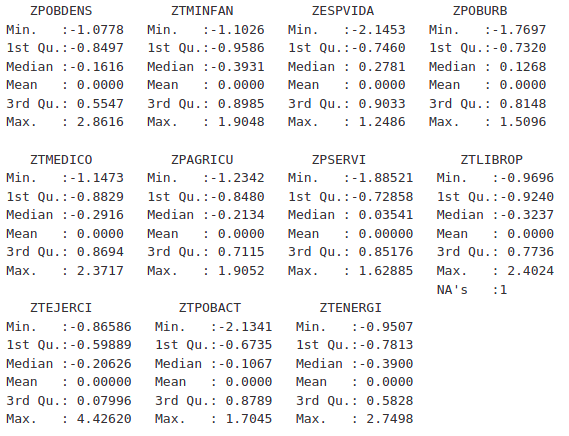
\includegraphics[scale=0.5]{img1.png}
    	    \caption{Se presentan información estadísticas sobre las variables del problema. Esta información incluye: valor mínimo y máximo, media, mediana, primer y tercer cuantil y existencia o no de valores perdidos.}
    	    \label{img1}
    	\end{figure}
	
	\subsection{Métodos estadísticos} 
	
    	Las técnicas estadísticas empleadas han sido: 
    	
    	\begin{itemize}
    
    	    \item Exploración descriptiva: Estudio de las distribuciones de las variables unidimensionales
    	    \item Exploración gráfica usando boxplots: para eliminación de outliers
    	    \item Método gráficos de comparación de cuantiles, qqplot: para comprobar la normalidad de las variables de manera visual
    	    \item Test de Kolmogorov-Smirnov: para comprobar la normalidad de las variables.
    	    
    	    \item Análisis de correlaciones: para comprobar qué variables están correladas y con cuales
    	    \begin{itemize}
    	        \item Test de Barlett
    	    \end{itemize}
    	    \item Test de Henze-Zirkler: para determinar si hay normalidad multivariante en la muestra
    	    \item Test de Mardia: igual que el anterior
    	    \item Test de Box M.: para contrastar la hipótesis \textit{La matriz de covarianzas es constante en todas las clases.}
    	    \item Análisis de Componentes Principales: Para reducir la dimensión de los datos
        	    \begin{itemize}
            	    \item Regla de Abdi et al.: Para obtener las componentes principales
            	    \item Scree Plot con el método del Codo: Para comprobar la validad de la Regla anterior
        	    \end{itemize}
    
    	    \item Análisis Factorial: Para reducir la dimensionalidad.
        	    \begin{itemize}
            	    \item Scree Plot con el método del codo: Para obtener el número óptimo de factores
            	    \item Análisis paralelo: Igual al anterior
                    \item Test de hipótesis: Igual a los anteriores. 
        	    \end{itemize}
        	    
    	    \item Análisis discriminante: Para clasificación
    	\end{itemize}
    	
	
	\section{Resultados}

    \subsection{Análisis univariante}

    	
    	En este análisis se ha encontrado un valor perdido en el atributo \textit{Ztlibprop} que representa el 3\% de la cantidad total y se ha sustituido por la media de dicho atributo. Las medidas resistentes de centralidad de casi todas las variables están desplazadas ligeramente a la izquierda a excepción de \textit{Zpservi, Zpesvida y Zpoburbs}, que están suavemente desplazada hacia la derecha. Tenemos también que todas las variables son platicúrticas a excepción de \textit{Zpobdens, Ztjerci y Ztenergi} que son leptocúrticas. Además, \textit{Ztenergi, Ztejerci, Ztlibrop, Zpagricu, Ztmedico, Ztminfan y Ztpobdens} tienen una cola simétrica extendida hacia los valores positivos mientras que el resto la tienen extendida hacia los valores negativos. También se ha detectado la presencia de outliers en los atributos \textit{Zpobdens y Ztejerci} y se han sustituido por la media puesto que no hay suficientes datos como para eliminarlos. \\ 
    	
    	Finalmente, se ha comprobado también que todas las variables siguen distribuciones normales univariantes de manera visual usando el método gráfico de comparación de cuantiles. Para el atributo \textit{Ztejerci} el método anterior generaba cierta controversia, por lo que se empleó el test de Kolmogorov-Smirnov. En dicho test se ha obtenido un p-valor de 0.02069, por tanto al 95\% de confianza se rechaza la hipótesis nula y la distribución no sigue una distribución normal. Pero se si aumenta el nivel de confianza hasta el 99\% no se puede rechazar dicha hipótesis y por tanto se podría admitir la normalidad.  \\

       \begin{figure}[H]
           \centering
           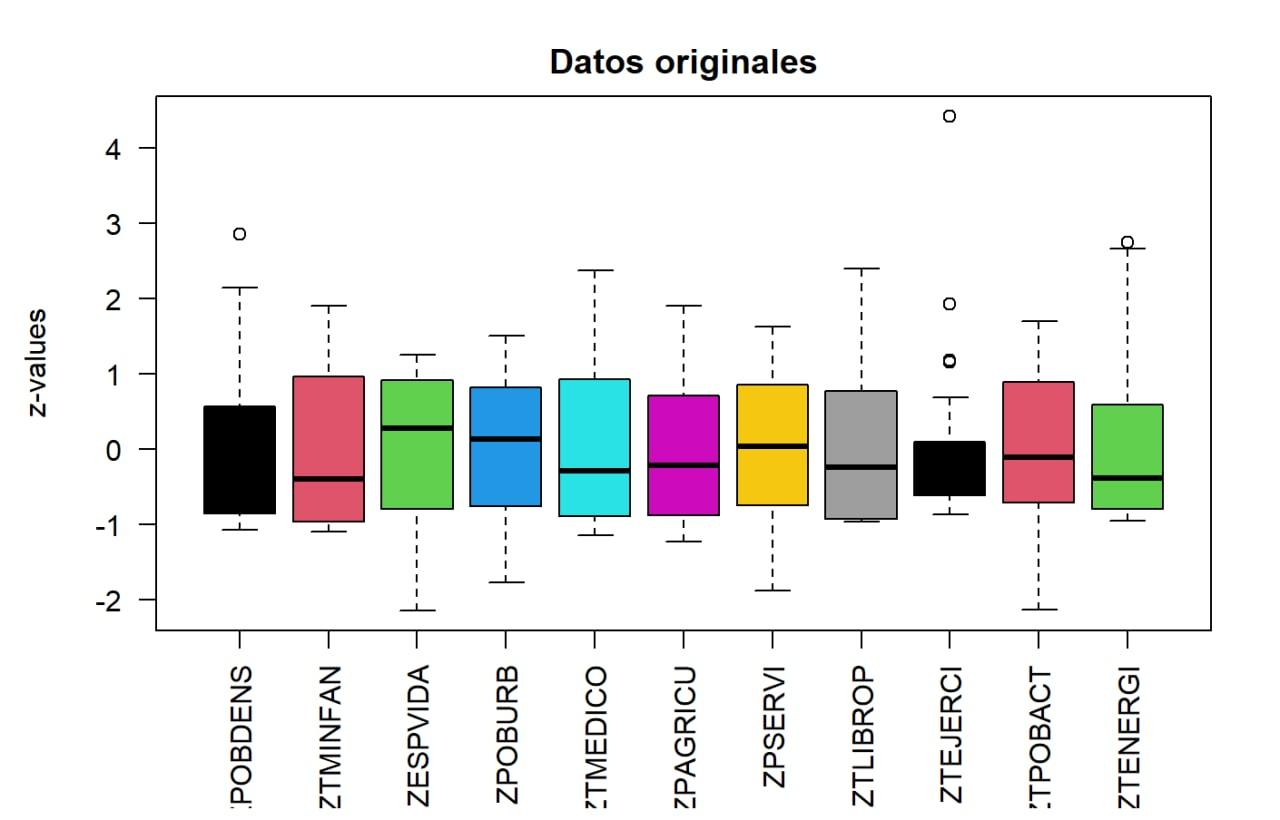
\includegraphics[scale=0.7]{img4.jpg}
           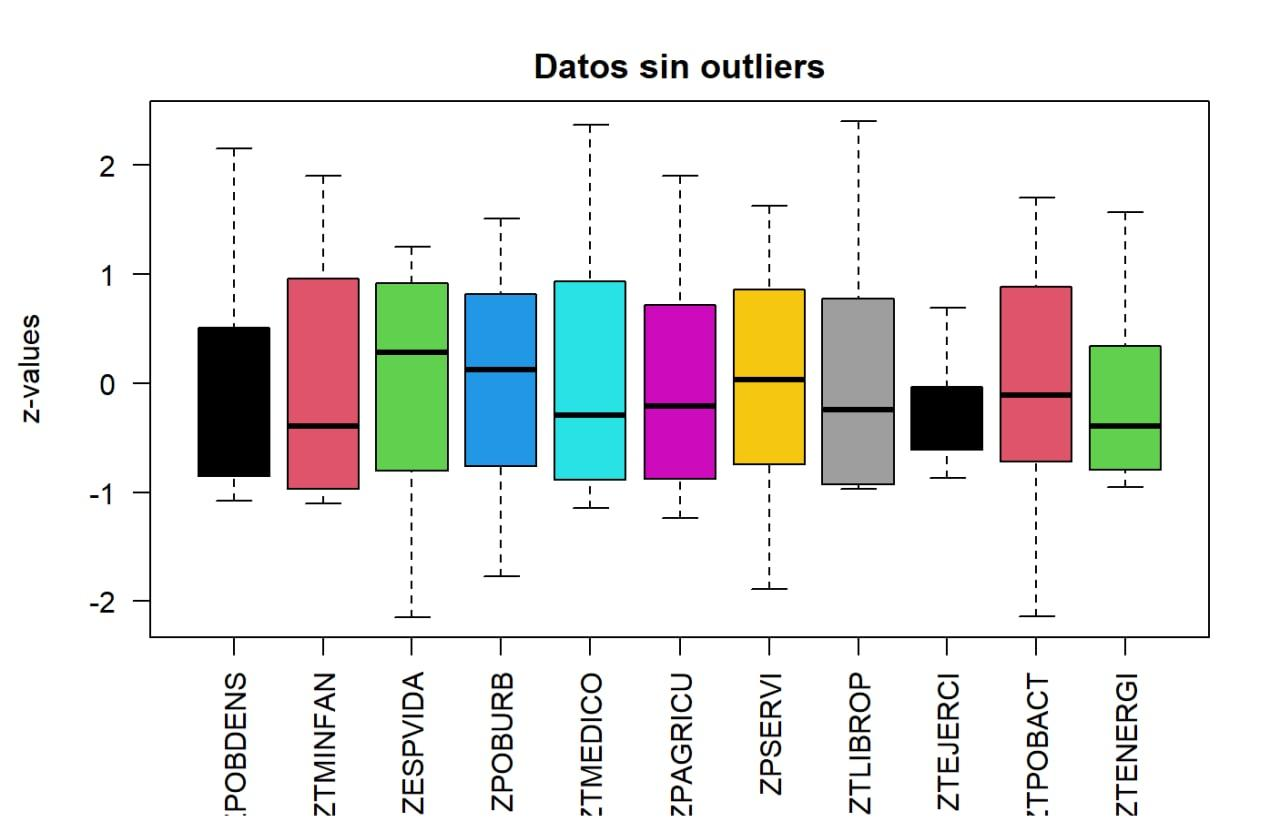
\includegraphics[scale=0.7]{img5.jpg}
           \caption{BoxPlots. En la imagen superior se muestran con los outliers y en la inferior sin ellos}
           \label{fig_1}
       \end{figure}
       
       \begin{figure}[H]
           \centering
           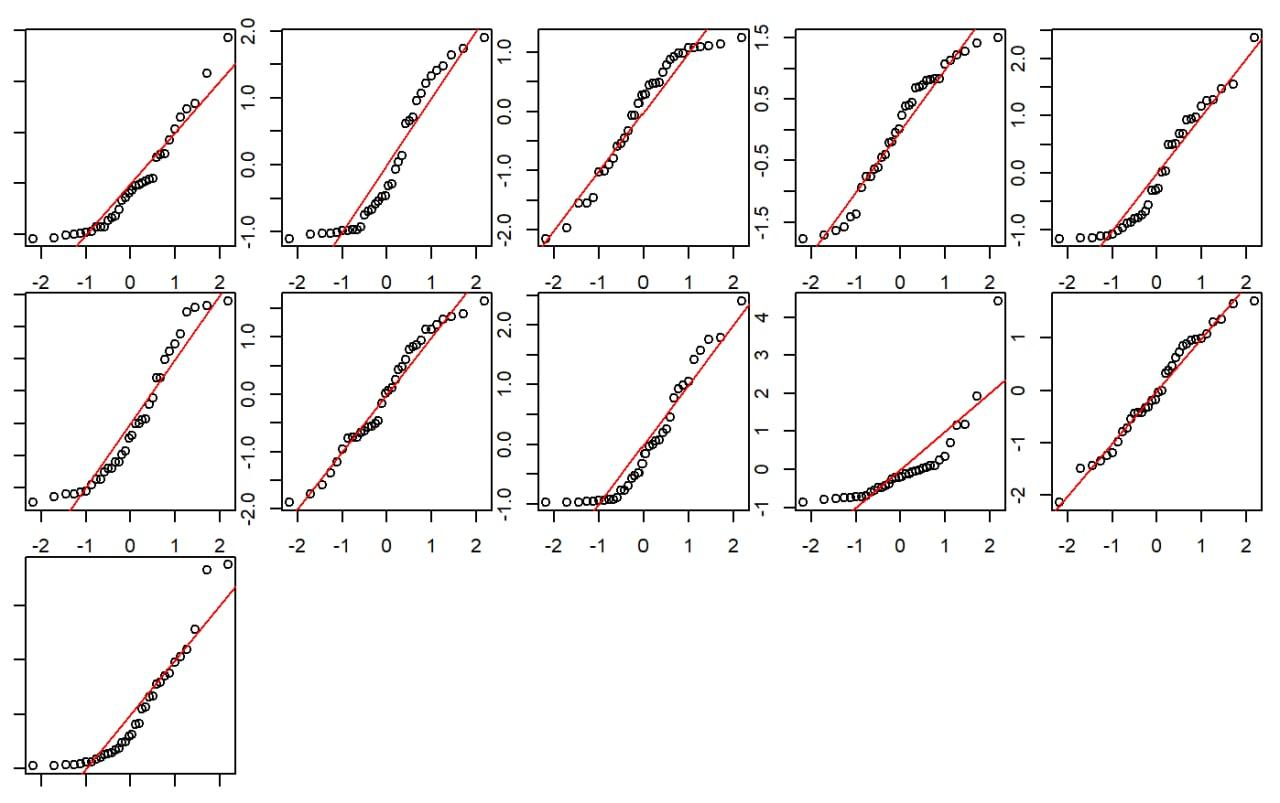
\includegraphics[scale=0.7]{img6.jpg}
           \caption{Gráficas generadas al aplicar a las variables el método gráfico de comparación de cuantiles qq-plot. Se observa de manera visual que todas las variables siguen una normal a excepción de la novena, que no queda muy clara.}
           \label{fig_2}
       \end{figure}

    \subsection{Análisis de componentes principales (ACP)}
    
    Para llevar a cabo un análisis de componentes principales es necesario que haya correlación entre las variables. Con el fin de determinar esto representamos la matriz de correlaciones:
    
            	\begin{figure}[H]
    	    \centering
    	    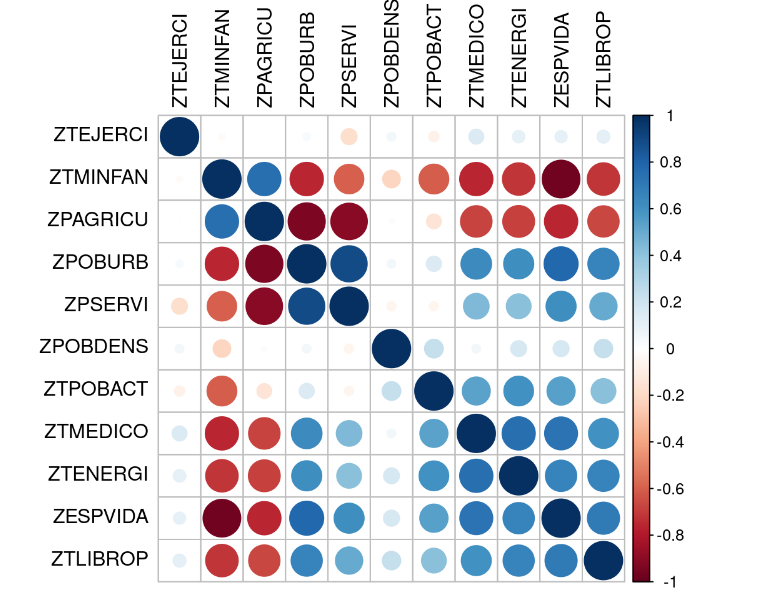
\includegraphics[scale=0.5]{cor.png}
    	    \caption{Matriz de correlaciones}
    	    \label{cor}
    	\end{figure}
    	
    	            	\begin{figure}[H]
    	    \centering
    	    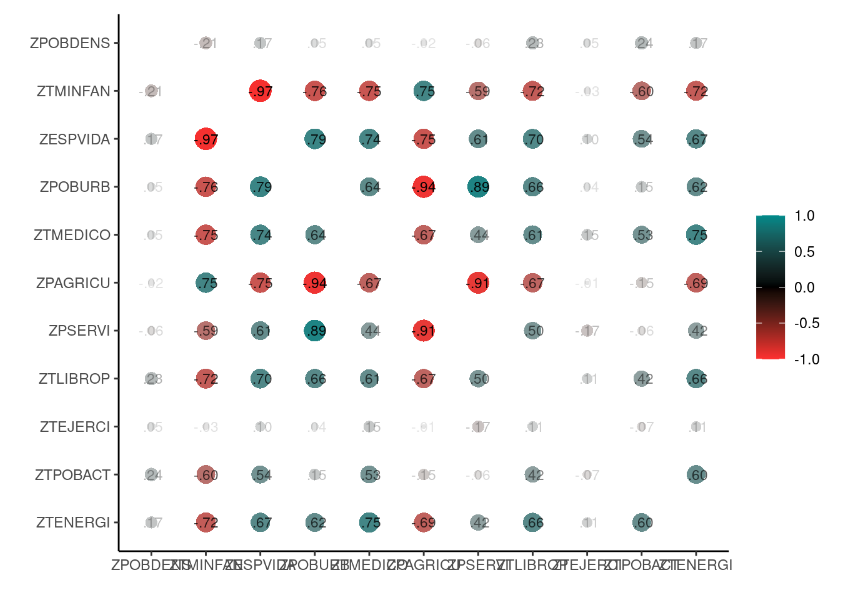
\includegraphics[scale=0.5]{cor2.png}
    	    \caption{Matriz de correlaciones}
    	    \label{cor2}
    	\end{figure}
    	
    Hay cierta correlación entre las variables, ya que la matriz de correlaciones dista de la matriz identidad. Por ejemplo vemos que la variable ZTMINFAN está correlada con la variable ZESPVIDA en un 96.7\% o la variable ZPAGRICU con ZPOBURB en un 93.8\%.  
    
    Para comprobar que a nivel poblacional efectivamente están correladas las variables usamos el test de Bartlett. El resultado del mismo nos lleva a rechazar la hipótesis nula, es decir, que las variables son incorreladas, de manera que podemos concluir que las variables están correladas y tiene sentido realizar un análisis de componentes principales. 
    
    Tras llevar a cabo un análisis de componentes principales se obtienen 11 componentes, cuya desviación típica, y varianza acumulada se muestran en la siguiente imagen:
    
        	\begin{figure}[H]
    	    \centering
    	    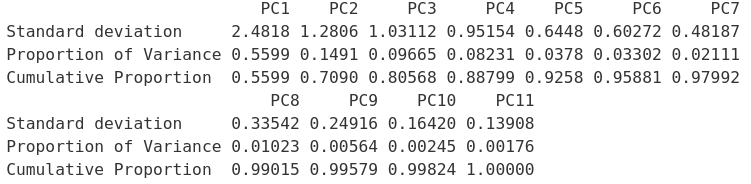
\includegraphics[scale=0.6]{componentes.png}
    	    \caption{Componentes principales obtenidas}
    	    \label{componentes}
    	\end{figure}
    Vemos a continuación la varianza explicada y varianza acumulada gráficamente. 
    
         	\begin{figure}[H]
    	    \centering
    	    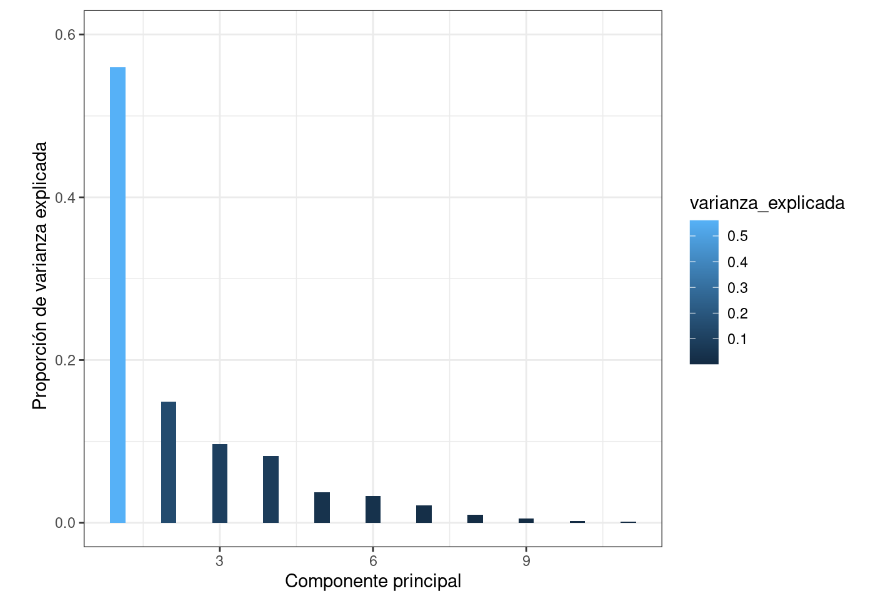
\includegraphics[scale=0.5]{varexp.png}
    	    \caption{Varianza explicada}
    	    \label{varexp}
    	\end{figure}
    	
    	         	\begin{figure}[H]
    	    \centering
    	    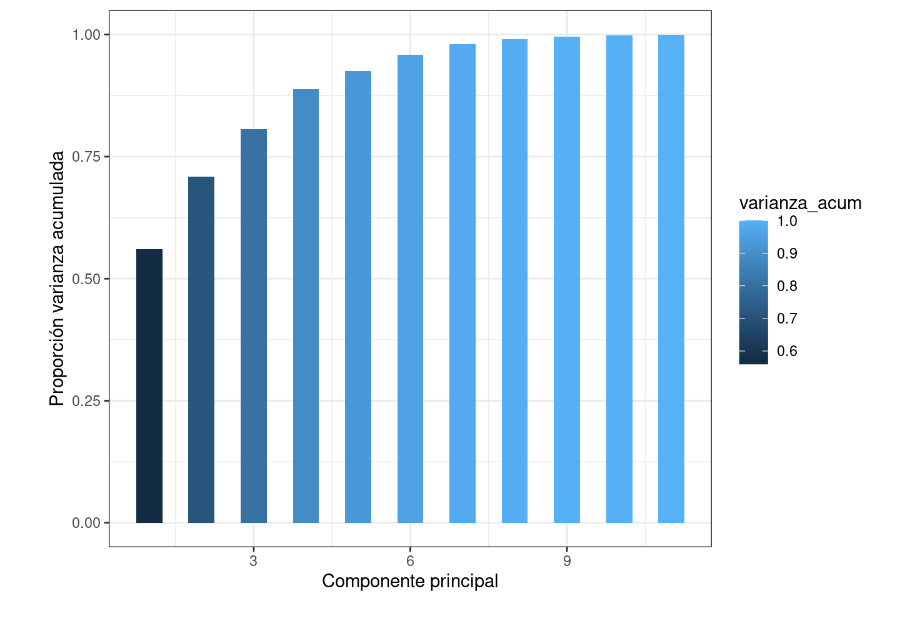
\includegraphics[scale=0.5]{varacum.png}
    	    \caption{Varianza acumulada}
    	    \label{varacum}
    	\end{figure}
    	
    	
    Para elegir el número óptimo de componentes principales usamos la regla de Abdi et al. (2010). La media en nuestro caso es 1, por estar las variables tipificadas, y obtenemos 3 componentes principales con una proporción de varianza explicada por cada una de ellas superior a 1, de manera que nos quedamos con las tres primeras componentes principales. La varianza acumulada es 0.8056758, luego estas componentes pricipales explican el 80,57\% de la varianza total. 
    
    Además de esta regla, usaremos una técnica gráfica. En concreto aplicamos el método del codo con ScreePlot: 
    
       	\begin{figure}[H]
    	    \centering
    	    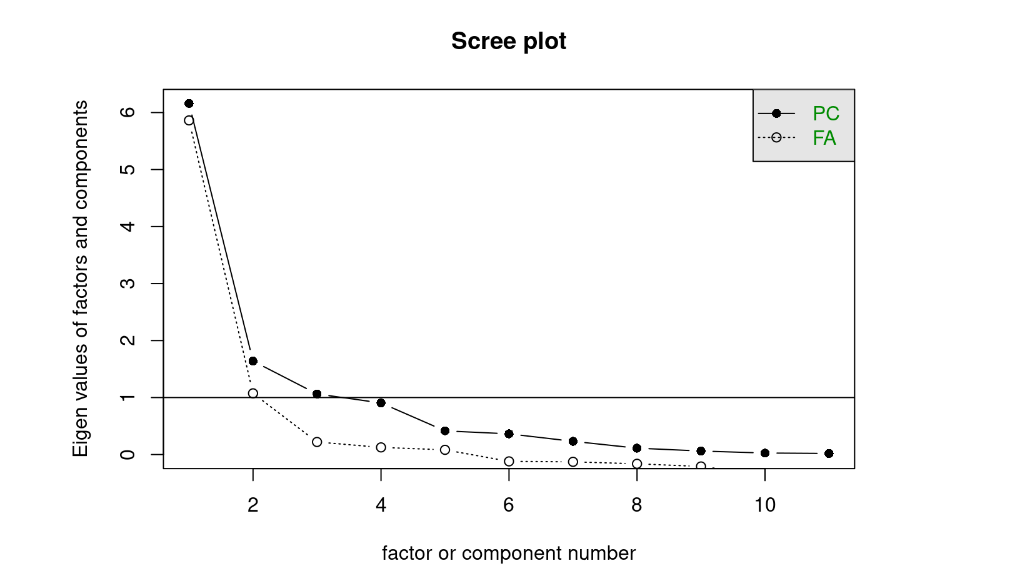
\includegraphics[scale=0.4]{codo1.png}
    	    \caption{}
    	    \label{codo}
    	\end{figure}
    
    Esta técnica confirma que el número de componentes principales a considerar debería ser 3. 
    
    Nos quedamos entonces con tres componentes principales, y se muestran a continuación tres gráficos donde se representan conjuntamente las variables y las observaciones relacionando visualmente las posibles relaciones entre las observaciones, las contribuciones de estas a las varianzas de las componentes y el peso que tienen las variables en la definición de las componentes principales:
    
    \begin{figure}[H]
    	    \centering
    	    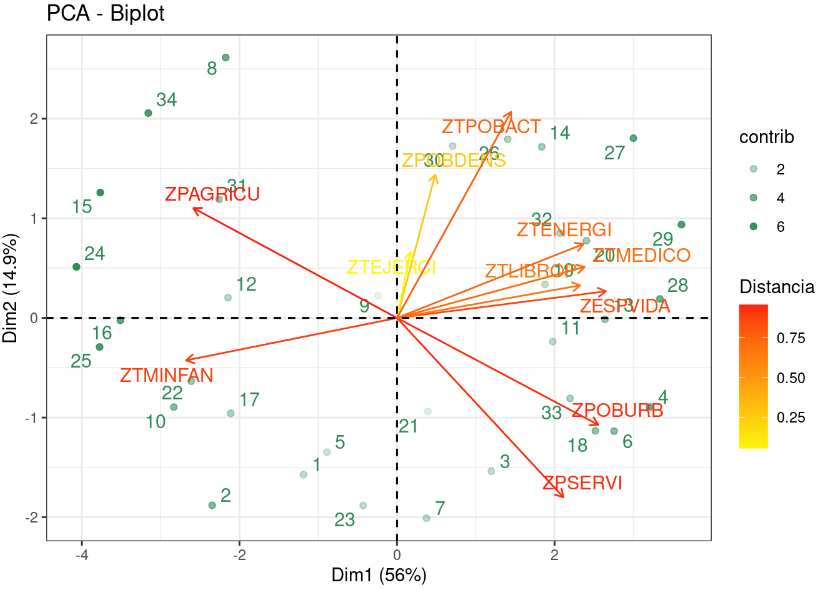
\includegraphics[scale=0.5]{pca4.png}
    	    \caption{Variables y observaciones en la 1º y 2ª componente principal}
    	    \label{pca4}
    	\end{figure}
    	
    	Vemos que algunas variables como ZPSERVI o ZTPOBACT están casi correladas por igual con ambas componentes principales. Sin embargo, hay muchas que están más correladas con la primera componente principal como ZTLIBROP, ZTMEDICO y ZESPVIDA, siendo esta última la que presenta una mayor correlación positiva con dicha componente principal, mientras que ZTMINFAN presenta una mayor correlación negativa con la primera componente. Por otro lado tenemos un par de variables, ZTEJERC y ZPOBDENS, que están más correladas con la segunda componente principal.
    	
    	Notamos que la observación que menos influye en la varianza explicada es la 9 pues está prácticamente sobre el origen de coordenadas. Las observaciones que más afectan a la primera componente principal son la 24 y la 29, ya que están más en los extremos del eje horizontal. Por otra parte, en la segunda componente principal, tienen más peso la observación 7 y 8.
    	
    	
     \begin{figure}[H]
    	    \centering
    	    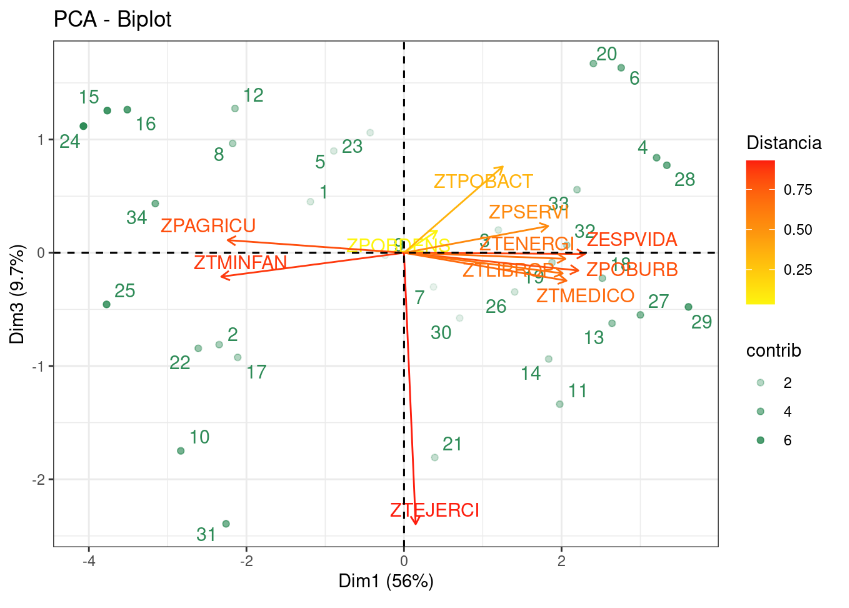
\includegraphics[scale=0.5]{pca5.png}
    	    \caption{Variables y observaciones en la 1º y 3ª componente principal}
    	    \label{pca5}
    	\end{figure}
    	
    
    
    	En este caso la mayoría de las variables están más correladas con la primera 
       componente principal, tanto positiva como negativamente. Unicamente vemos una 
    	variable, ZTEJERCI que está casi perfectamente correlada negativamente con la 
    	tercera componente principal. Apreciamos además una variable, ZTPOBACT, que    	
   	presenta prácticamente la misma correlación positiva con ambas componentes   	
    	principales. Además, notamos que hay una mayor correlación de las variables con la primera componente principal respecto a la tercera de la que había con la primera
    	componente con respecto a la segunda en el primer gráfico, ya que las flechas están más pegadas al eje horizontal.
    	

    	
    	En este caso observamos que los datos 9 y 7 son los que menos afectan a las primera y tercera componente principal. Al igual que observamos en el gráfico anterior, los datos 29 y 24 son los que mayor influencia tienen en la primera componente, mientras que las observaciones 20 y 31 afectan en mayor medida a la tercera componente.
    	
         \begin{figure}[H]
    	    \centering
    	    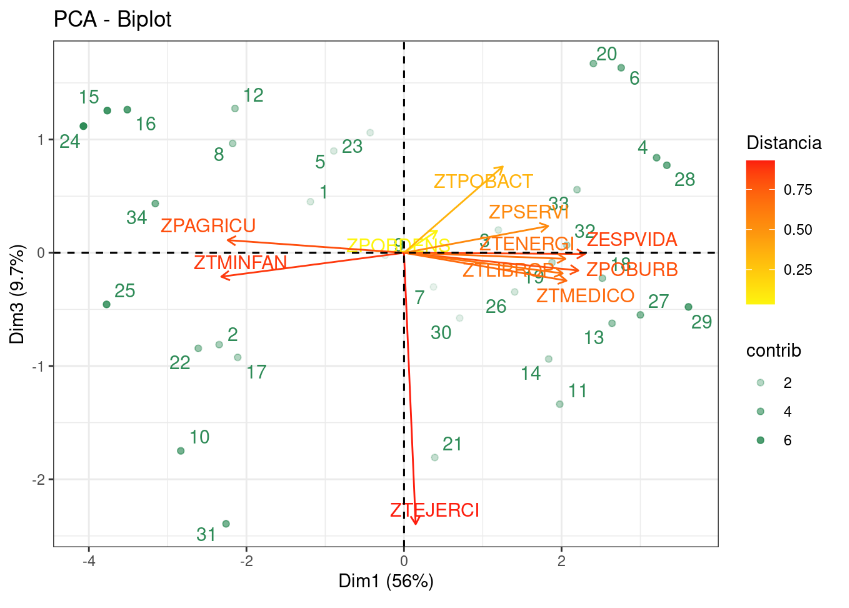
\includegraphics[scale=0.5]{pca5.png}
    	    \caption{Variables y observaciones en la 2ª y 3ª componente principal}
    	    \label{pca6}
    	\end{figure}
    	
    	Como ocurría en el caso anterior, solo la variable ZTEJERCI está fuertemente correlada con la tercera componente principal, aunque aquí esta variable tiene algo más de peso en la segunda componente principal de la que tenía en la primera. Vemos que el resto de variables están más correladas con la segunda componente principal, aunque en general no en gran medida, pues las flechas son pequeñas y de color oscuro. La variable ZTPOBACT, al igual que en el gráfico anterior, influye casi por igual en ambas componentes principales, siendo en este gráfico la correlación positiva mayor, pues la flecha es de mayor longitud.
    	
    	La observación 9 vuelve a ser la que menos afecta a las componentes principales, seguida de la 19 y la 13. La segunda componente se ve más influenciada, como ya sabíamos, por las observaciones 7 y 8. Con respecto a la tercera componente, el dato 31 es el más influyente, seguido por el 20, lo cual coincide con lo visto en el gráfico anterior.
     
    \subsection{Análisis Factorial (AF)}
    
    Para determinar el número óptimo de factores a considerar usaremos dos técnicas gráficas (scree plot y análisis paralelo) y un test de hipótesis (factanal). Mostramos en primer lugar los resultados de las técnicas gráficas:
    
    \begin{figure}[H]
    	    \centering
    	    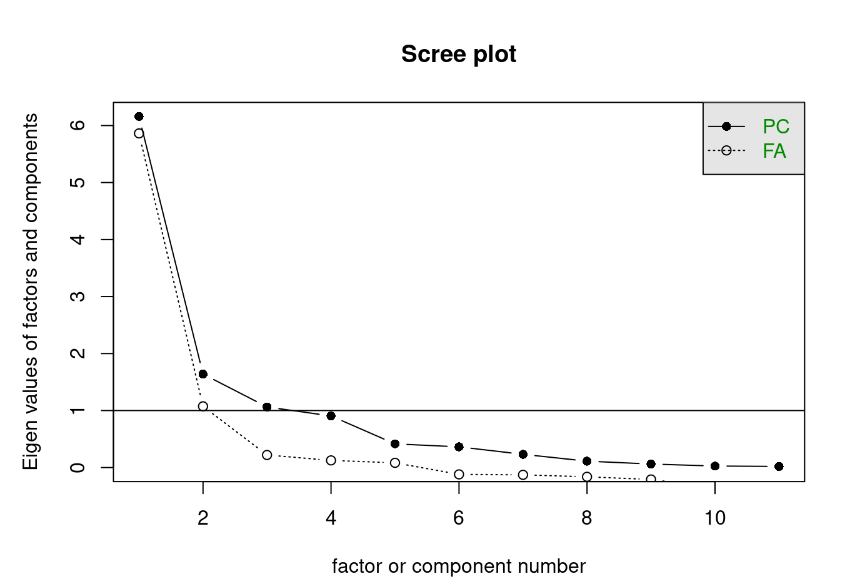
\includegraphics[scale=0.5]{screeplot2.png}
    	    \caption{Scree plot}
    	    \label{plot2}
    	\end{figure}
    	
    Por el método del codo deducimos que el número de factores a considerar debería estar entre 2 y 3. 
             \begin{figure}[H]
    	    \centering
    	    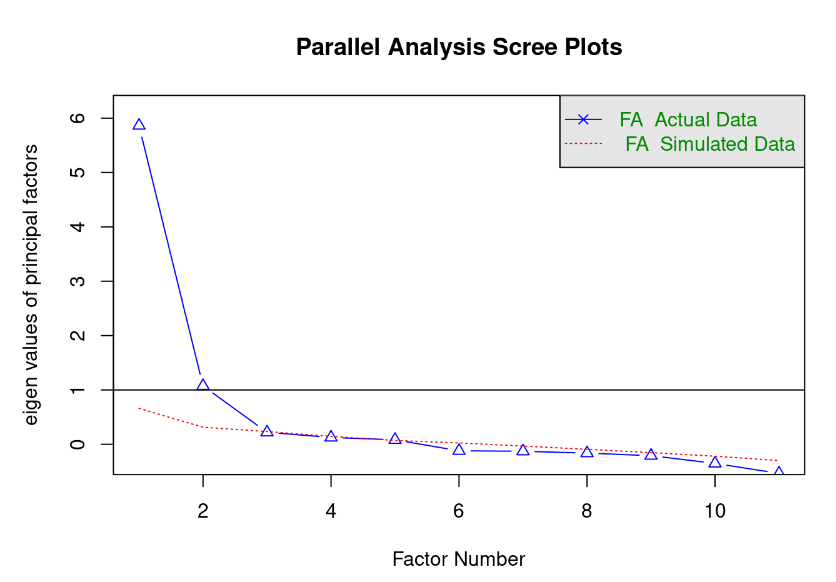
\includegraphics[scale=0.5]{parallel analysis.png}
    	    \caption{Análisis paralelo}
    	    \label{plot3}
    	\end{figure}
    	
    El análisis paralelo indica que hay al menos dos factores, siendo posible considerar un tercer factor, pues la línea de puntos del análisis paralelo cruza la línea sólida del análisis factorial en el tercer factor, o incluso en el cuarto y quinto.
    
    El test de hipótesis indica que 2 factores no son suficientes, pero 3 sí que lo son, de modo que tomaremos 3 factores para llevar a cabo el análisis factorial.
    
    Así pues, estimamos el modelo factorial con 3 factores usando una rotación con el enfoque \textbf{varimax}. \\ 
    
    La matriz de pesos factorial obtenida , así como la proporción de varianza explicada y acumulada para cada factor,  ha sido la siguiente:
    
                 \begin{figure}[H]
    	    \centering
    	    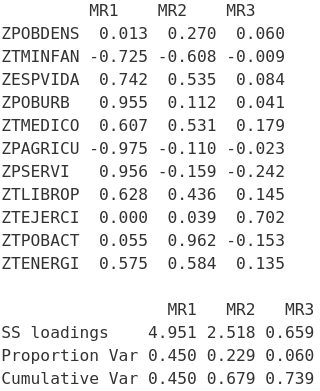
\includegraphics[scale=0.5]{af.png}
    	    \caption{Resultados del análisis factorial}
    	    \label{af}
    	\end{figure}
    	
    La varianza acumulada explicada es de 0.739, es decir, el 74\% de la varianza original queda explicada por los tres factores determinados. 
    

    Ahora mostramos gráficamente con qué variables correlaciona cada uno de los factores obtenidos: 
    
                     \begin{figure}[H]
    	    \centering
    	    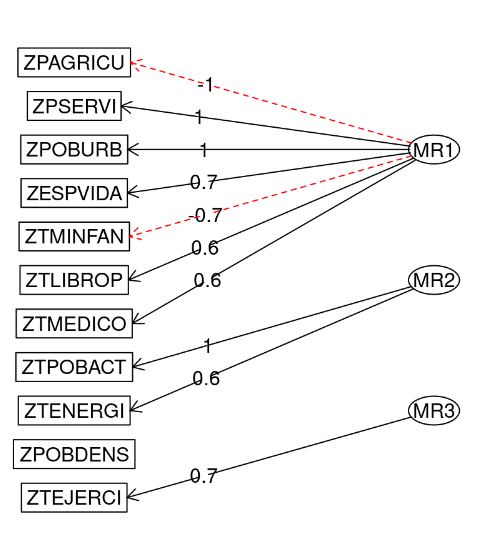
\includegraphics[scale=0.45]{plotaf.png}
    	    \caption{}
    	    \label{plotaf}
    	\end{figure}
    	
    Podemos ver que el primer factor tiene una alta correlación con un gran número de variables, tanto de forma positiva como negativa. En cambio, el segundo factor sólo se correlaciona en gran medida con dos variables, ZTPOBACT y ZTENERGI, siendo la correlación con la variable ZTPOBACT perfecta y positiva. El tercer factor tiene una correlación alta únicamente con una variable, ZTEJERCI. Hay una variable, ZPOBDENS, que presenta correlación baja con los tres factores. \\
    
    
     Notamos además que, el hecho de aplicar una rotación ortogonal, ha permitido que estemos cerca de una situación ideal, en la que tendríamos una alta correlación de cada uno de los factores con un grupo de variables observables concretas y prácticamente nula con el resto. Podemos ver por ejemplo que la variable observable ZTEJERCI tiene una alta correlación con el tercer factor y casi nula con los otros dos factores. Lo mismo ocurre con ZTPOBACT, que está casi perfectamente correlada con el segundo factor y presenta una correlación baja con el resto de factores. El primer factor tiene una alta correlación con un grupo mayor de variables observables, siendo por ejemplo la correlación casi perfecta con las variables ZPSERVI, ZPAGRICU y ZPOBURB, las cuales no presentan a penas correlación con los otros factores. \\


    
    \subsection{Análisis discriminante}

    	Para realizar este análisis hemos tenido que etiquetar los datos. Se ha etiquetado de forma binaria a las instancias dividiendo a las que tienen el valor del atributo \textit{ZespVida} por encima de la mediana de los que los tienen por debajo. \\

        \begin{figure}[H]
            \centering
            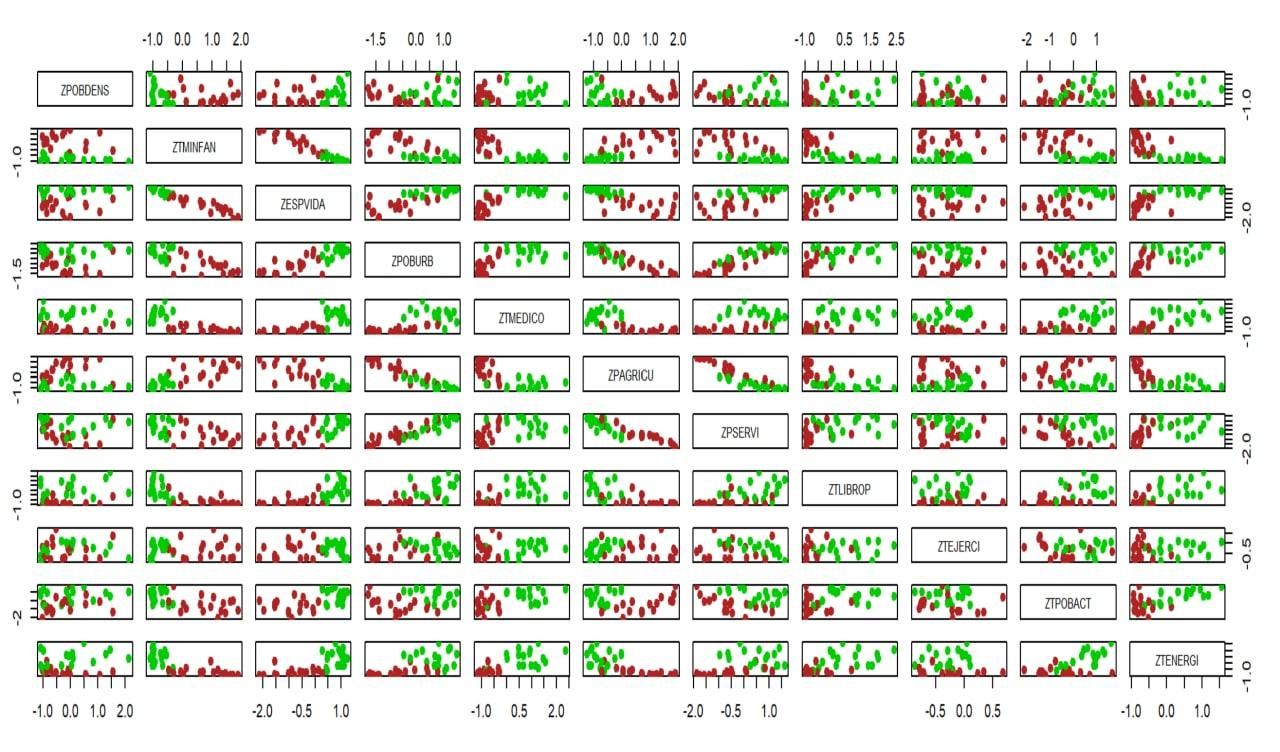
\includegraphics[scale = 1]{img7.jpg}
            \caption{Separación de clases entre pares de variables}
            \label{fig:my_label}
        \end{figure}

    	También, es necesario que haya normalidad multivariante en los datos. Para comprobarlo se usan los tests de  \textit{Henze-Zirkler} y de \textit{Mardia}. Ambos tests muestran evidencias para suponer que hay normalidad multivariante al 95\% de confianza. Por otra parte es necesario contrastar la hipótesis de que la matriz de covarianzas es constante en todas las clases y para ello se usa el Test de \textit{Box M}, dicho test es sensible a que los datos se distribuyan según una normal multivariante, que efectivamente se cumple. El resultados del test nos da un p-valor menor que 0.001 y rechazamos entonces la hipótesis nula, esto es, asumimos la no homogeneidad de varianzas, por lo que es recomendable usar un análisis discriminante cuadrático (QDA), aunque también se ha hecho el lineal (LDA).\\ 
    	
        En las tablas \ref{tabla1} y \ref{tabla2} presentamos los resultados del entrenamiento en forma de matriz de confusión. El \textit{error de entrenamiento} para LDA es de 0\% mientras que para QDA es de aproximadamente un 2.9\%. Ambos modelos presentan una probabilidad a priori del 50\%. 
    	
    	\begin{table}[H]
        \caption{QDA: Resultados entrenamiento}
        \begin{center}
        \begin{tabular}{|l|r|r|}
        \hline
        \textbf{QDA} & \multicolumn{1}{l|}{\textbf{a}} & \multicolumn{1}{l|}{\textbf{b}} \\ \hline
        \textbf{a} & 17 & 0 \\ \hline
        \textbf{b} & 1 & 16 \\ \hline
        \end{tabular}
        \end{center}
        \label{tabla1}
        \end{table}
        
        \begin{table}[H]
        \caption{LDA: Resultados entrenamiento}
        \begin{center}
        \begin{tabular}{|l|r|r|}
        \hline
        \textbf{LDA} & \multicolumn{1}{l|}{\textbf{a}} & \multicolumn{1}{l|}{\textbf{b}} \\ \hline
        \textbf{a} & 17 & 0 \\ \hline
        \textbf{b} & 0 & 17 \\ \hline
        \end{tabular}
        \end{center}
        \label{tabla2}
        \end{table}
        
        Se creó un nuevo registro para clasificarlo con los siguientes valores: \textit{ZPOBDENS=0.3, ZTMINFAN=-0.2, ZESPVIDA=0.1, ZPOBURB=-0.1, ZTMEDICO=0.5, ZPAGRICU=-0.5, ZPSERVI=0.5, ZTLIBROP=0.3, ZTEJERCI=-0.8, ZTPOBACT=0.2, ZTENERGI=0.1}. Los resultados se muestran en la tabla \ref{tabla3}. \\   
        
        \begin{table}[H]
        \caption{Predicción }
        \begin{center}
        \begin{tabular}{|l|l|l|}
        \hline
        \textbf{} & \textbf{a} & \textbf{b} \\ \hline
        \textbf{LDA} & 0.003296763 & 0.9967032 \\ \hline
        \textbf{QDA} &  0.917501 & 0.08249898 \\ \hline
        \end{tabular}
        \end{center}
        \label{tabla3}
        \end{table}
        
        \begin{figure}[H]
            \centering
            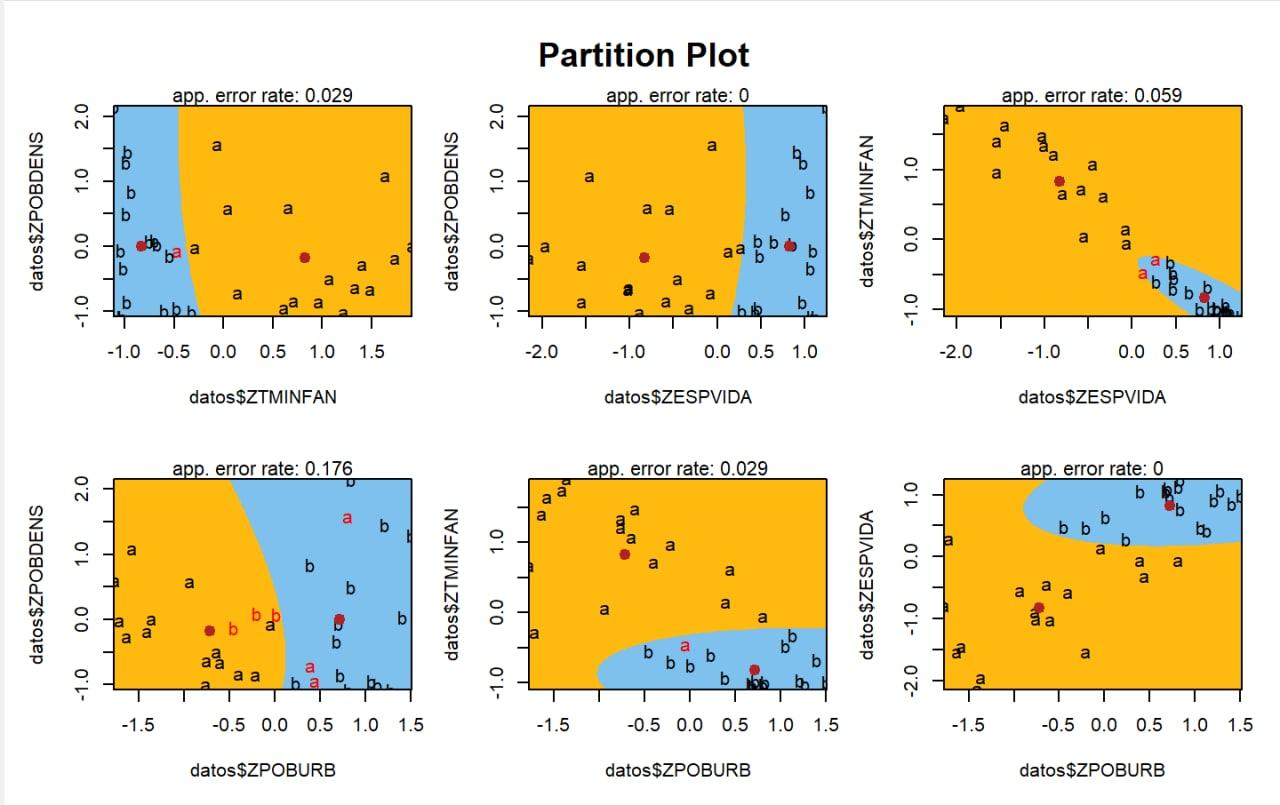
\includegraphics[scale=1]{img2.jpg}
            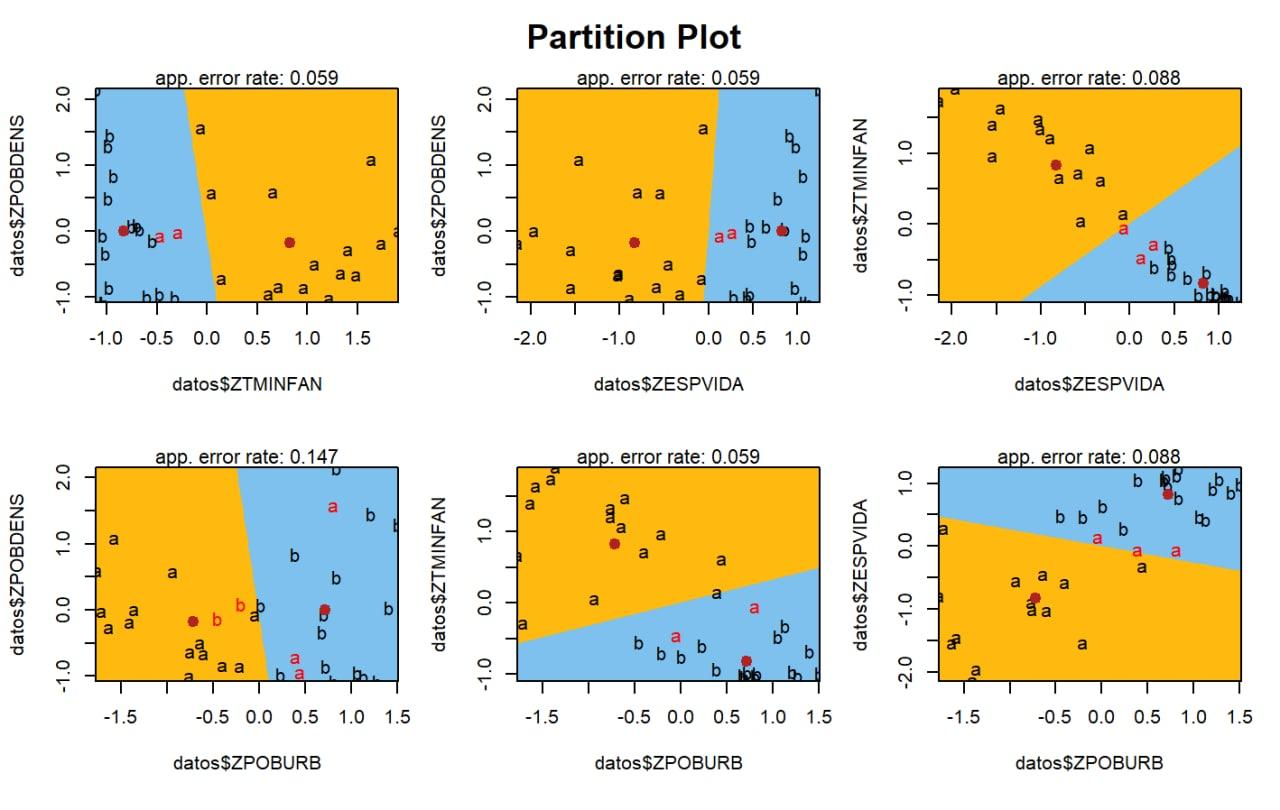
\includegraphics[scale=1]{img3.jpg}
            \caption{Representación de los límites del modelo para cada par de predicciones. Cada color representa una región de clasificación acorde al modelo, se muestra el centroide de cada región y el valor real de las observaciones. La imagen superior corresponde al QDA y la inferior al LDA }
            \label{img2}
        \end{figure}
        
    


        


	
	\section{Discusión}
	
    El objetivo del trabajo como ya hemos mencionado, consiste en descubrir patrones, perfiles y tendencias a partir del análisis de los datos utilizando las técnicas estadísticas del análisis multivariante de datos aprendidas a lo largo del curso. \\ 
    
	En efecto, en el \textbf{\underline{Análisis Univariante}} podemos interpretar que todas las variables se distribuyen según una normal univariante, siendo una de ellas un poco conflictiva. \\ 
	
    De los resultados obtenidos para el \textbf{\underline{análisis de componentes principales}}, podemos decir, viendo las Figuras 8, 9 y 10 que la componente principal con la que están menos correladas las variables es la tercera, siendo únicamente ZTEJERCI la variable que más peso tiene en la tercera componente, aunque el resto también influyen, como por ejemplo, ZTPOBACT, que tiene un peso considerable en dicha componente. El resto de variables tienen, en general, más peso en la primera componente, aunque su influencia en la segunda también es considerable, estando algunas variables más correladas con la segunda que con la primera. \\
    
    Además, podríamos considerar eliminar la observación 9 para este análisis, pues no parece afectar a las componentes principales seleccionadas. Por su parte, la observación 31 parece decisiva en la elección de la tercera componente principal. El resto de datos afectan por igual a la primera y segunda componente, con algunas excepciones de datos extremos que influyen en mayor medida en una u otra, como por ejemplo la observación 7, con gran peso en la segunda pero casi nulo en la primera. \\
    
    Por su parte, en el \textbf{\underline{análisis factorial}} el primer factor es el que está más correlacionado con la mayoría de las variables. Los otros dos factores están poco correlacionados con casi todas las variables, sobre todo el tercero, el cual vimos que sólo está correlacionado de manera considerable con una variable y su correlación con el resto de variables es prácticamente nula. Este hecho explica que, a la hora de seleccionar el número de factores óptimos estuviéramos en duda entre 2 y 3, pues el tercero parece aportar poco. De hecho, la proporción de varianza explicada del mismo es solamente del 6\%. \\
    
   
    
    Si comparamos PCA con AF, en ambos casos hemos concluido que el número de componentes y factores óptimos a considerar era de 3. Sin embargo, las componentes principales explicaban un mayor porcentaje de la varianza total que los factores de AF, 80,57\% frente a 74\%. Además, con AF teníamos una variable, ZPOBDENS, que casi no estaba correlacionada con ninguno de los factores obtenidos. Así pues, podemos decir entonces que PCA obtiene en este caso mejores resultados, por lo que si tuviéramos que elegir entre reducir la dimensionalidad con PCA frente a AF, quizás sería más conveniente elegir PCA. \\
	



	Por una parte, el \textbf{\underline{análisis discriminante}} mediante QDA presenta un error de entrenamiento perfecto, del 0\%, esto es, el modelo se ajusta totalmente a los datos de entrenamiento. Mientras que el modelo de LDA se adapta también muy bien pero no es perfecto. Luego podemos incurrir en un posible sobreajuste, sobre todo en el QDA. Pese a que tenemos muy pocos ejemplos de entrenamiento, y los valores de las etiquetas han sido \textit{''inventados''} no podemos esclarecer con total seguridad lo anterior. Aunque en la figura (Fig. \ref{img2}) podemos ver por ejemplo que hay una partición en concreto en la que visualmente se produce sobreajuste (\textit{Zpobdens-Zespvida}). \\  
	
	Tras ingresar un nuevo registro, obtenemos que la clasificación por parte de ambos modelos da lugar a desconcierto. Pues cada uno afirma con casi total seguridad que pertenece a una etiqueta la cual es negada por el otro. Volviendo a reiterar lo anteriormente comentado, y al no tener constancia de qué etiqueta tiene realmente el registro inventado no podemos saber cual es la predicción errónea. Aunque, según el criterio usado para etiquetar, es más lógico la etiqueta que predice QDA, puesto que el valor de \textit{Zespvida} está por debajo de la mediana. \\
	
	
	\section{Conclusión}  
	
	En nuestro estudio hemos realizado un análisis univariante de los datos, sustituyendo tanto los outliers como los valores perdidos por la media. Este tratamiento que hemos hecho de los outliers puede que no sea el mejor, pues podrían eliminarse directamente, sustituirse por la mediana en lugar de la media, o trabajar con ellos sin modificarlos. Sería necesario analizar la naturaleza de los mismos para saber cómo lidiar con ellos de un modo más conveniente, pues puede ser que se deban simplemente a ruido en las mediciones, en cuyo caso sí que habría que eliminarlos,  o que realmente tengan importancia en la población y serían tratados con la misma importancia que el resto de los datos. \\
	
	Hemos conseguido reducir la dimensionalidad, tanto mediante variables observables (PCA) como mediante variables latentes (AF), pasando de las 11 variables originales a solamente 3, lo cual facilita la interpretabilidad. Con esta reducción perdemos parte de la varianza explicada, pues las 3 componentes principales explicarían el 80\% de la varianza, y, con las variables latentes, se explica el 74\%. Así, con PCA no se pierde demasiada varianza, pero con AF sí, de modo que dependiendo de la aplicación que se le quiera dar a los datos convendría realizar esta reducción o no. Por ejemplo, para clasificación con técnicas de Machine Learning (ML) la reducción de la dimensionalidad suele ser conveniente para dar mayor rapidez al entrenamiento y evitar el sobreajuste al reducir la varianza. \\

    En cuanto al análisis discriminante comentar que no tiene mucho sentido pues las etiquetas han sido inventadas y no tiene ningún tipo de validez ni de caso práctico. En su lugar, se debería de haber hecho con una base de datos etiquetada. Sin embargo, con nuestros datos hemos conseguido llevar a cabo una clasificación casi perfecta de los datos de entrenamiento, con un clasificador tanto lineal como cuadrático.\\
    
    Podría realizarse una clasificación con técnicas de Machine Learning más avanzadas para obtener mejores resultados y evitar sobreajuste, pero para esto necesitaríamos más datos, y etiquetas reales. Podría llevarse a cabo un aumento de los datos, modificando ligeramente los datos de los que disponemos con determinadas técnicas existentes en ML para aumentar el número de datos. 
    \\  
	
	

    \section{Anexo}
    
    Participación:
    
    \begin{itemize}
        \item Análisis univariante: Juanjo y Adrian
        \item ACP: Pilar 
        \item AF: Pilar y Adrián
        \item AD: Juanjo
        \item Memoria: Adrián, Pilar y Juanjo.
    \end{itemize}
    
    Lo parte que ha realizado cada uno es algo relativo, pues a lo largo del trabajo nos hemos ido constantemente retroalimentando, proponiendo ideas, corrigiendo erratas y verificando que lo que hizo cada uno era correcto. De este modo, aunque Pilar haya hecho el ACP, Adrían y Juanjo comprobaron que estaba todo correcto, así como también Pilar y Adrián comprobaron que el análisis discriminante no tuviera errores.

    
    
    
	
	
\end{document}